Having studied the vector space structure of $\R^n$ and the geometric behavior of linear maps, we will now turn our focus to studying  \textbf{non-linear}  functions from $\R^n$ to $\R^m$.  In particular, this will lead us to study the geometric and topological properties of $\R^n$. 

In section \ref{sec:multifunctions}, we will first explore functions $\R \to \R^n$ (\hyperref[vectorvaluedfunctions]{vector-valued functions}), as well as functions $\R^n \to \R$ (\hyperref[multivariablefunctions]{multivariable functions}).  These turn out to be enough to capture the behavior of \hyperref[generalmulti]{general multivariable functions} $\R^n \to \R^m$.

We will then study the notions of limits (section \ref{sec:limits}) and continuity  (section \ref{sec:continuity}) for these classes of functions, and see how it differs from limits and continuity in the single-variable case.


\section{Multivariable functions}\label{sec:multifunctions}

\subsection{Vector-valued functions}\label{vectorvaluedfunctions}

We will begin by studying vector-valued functions.  That is, maps of the form $f : \R \to \R^n$.  Note that the domain of $f$ is $\R$, so that the input of this function is a scalar.  On the other hand, the codomain of $f$ is $\R^n$, which means that the output is a point (position vector), hence the name vector-valued function. 

\begin{definition}
    A \textbf{vector-valued function}\define{vector-valued function} is a function $\bm{r}(t): \R \to \R^n$, given by
    $$\bm{r}(t) = \langle x_1(t),x_2(t), \cdots x_n(t) \rangle = x_1(t)\bm{e_1} + x_2(t)\bm{e_2} + \cdots + x_n(t)\bm{e_n}$$
    where all of the $x_i(t) : \R \to \R$ are single-variable functions.
    
    \vspace{1em}  
    $\bm{r}(t)$ is also called a \textbf{parametrization}\define{parametrization} (with \textbf{parameter} $t$).
    \end{definition}

In other words, vector-valued functions are precisely described by their component functions $x_i(t)$.  We will see that this will cause vector-valued functions $\bm{r}(t) : \R \to \R^n$ to behave extremely similarly to scalar functions $f : \R \to \R$.  In some sense, a vector-valued function $\bm{r}(t) : \R \to \R^n$ is simply a collection of $n$ single-variable scalar functions.
 \begin{center}        
        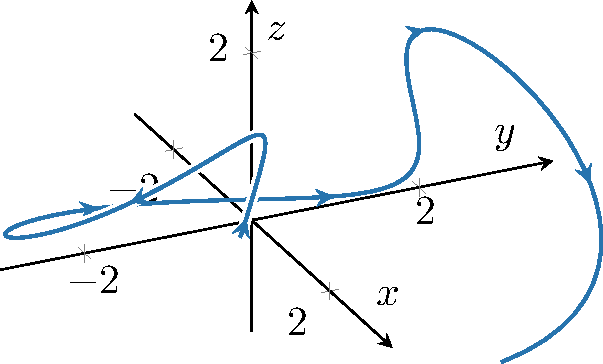
\includegraphics[scale=.75]{chapters/2-RealAnalysis/figures/figures-vectorval1.pdf}
    \end{center}

\begin{motivating}
How should we geometrically interpret vector-valued functions?
\end{motivating}

We should think of a vector-valued function $\bm{r}(t)$ as describing the motion of a particle in $\R^n$.  For example, let us think of the units of $t$ as begin seconds.  Then we can interpret the vector $\bm{r}(0)$ as describing the position of a particle at time $t=0$.  We can then think of the vector $\bm{r}(1)$ as describing the position of the particle 1 second after $t=0$; and similarly, the vector $\bm{r}(-1)$ describes the position of the particle 1 second \textbf{before} $t=0$.  

 \begin{center}        
        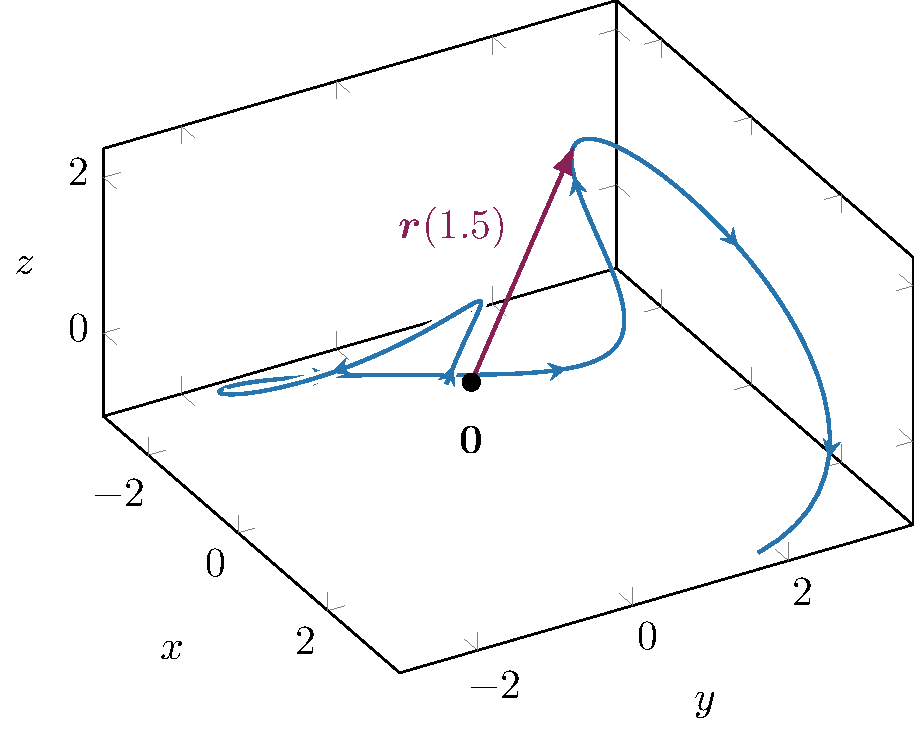
\includegraphics[scale=.75]{chapters/2-RealAnalysis/figures/figures-vectorvalpoint.pdf}
    \end{center}

Let us turn to some examples:

\begin{example}
A scalar function $f : \R \to \R$ is a vector-valued function for $n=1$.
\end{example}


\begin{example}
Sketch the vector-valued function $\bm{c}(t) = \langle  -\sin(t), \cos(t) \rangle$ in $\R^2$.

 \begin{center}        
        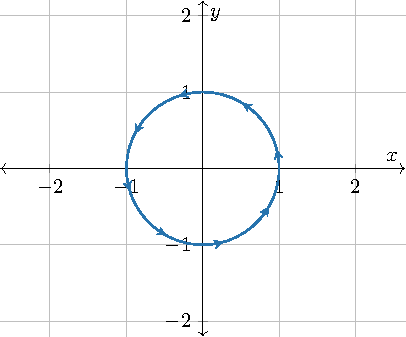
\includegraphics{chapters/2-RealAnalysis/figures/figures-vectorcircle.pdf}
    \end{center}

\end{example}


\begin{example}\label{helix1}
Sketch the vector-valued function $\bm{h}(t) = \langle -\sin(t), \cos(t), t \rangle$ in $\R^3$.

 \begin{center}        
        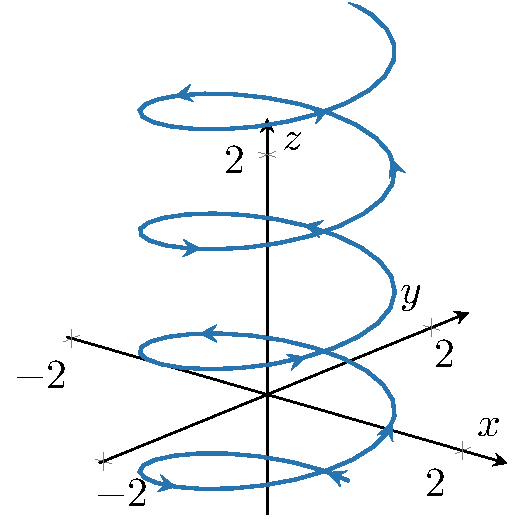
\includegraphics[scale=.75]{chapters/2-RealAnalysis/figures/figures-helix.pdf}
    \end{center}
\end{example}

\begin{example}\label{helix2}
Sketch the vector-valued function $\bm{r}(s) = \langle -\sin(5s), \cos(5s), 5s \rangle$ in $\R^3$.

 \begin{center}        
        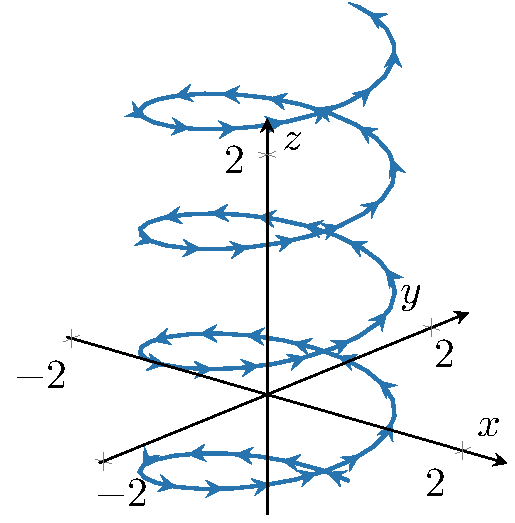
\includegraphics[scale=.75]{chapters/2-RealAnalysis/figures/figures-helix5x.pdf}
    \end{center}

\end{example}

\begin{motivating}
How do the two examples \hyperref[helix1]{$\bm{h}(t)$} and \hyperref[helix2]{$\bm{r}(s)$} differ from each other?
\end{motivating}

\begin{definition}

    Given a parametrization $\bm{r}(t) : \R \to \R^n$, we say that its \textbf{parametric curve}\define{parametric curve} is the set of points $$\{\bm{x} \in \R^n \ | \ \bm{x} = \bm{r}(t)\} \subset \R^n$$
    
\end{definition}

That is, we can geometrically interpret the parametric curve as being the path traced out by the parametrization $\bm{r}(t)$.  

\begin{example}
The parametric curve of $\bm{c}(t) = \langle  -\sin(t), \cos(t) \rangle$ is the circle of radius 1, centered at the origin.

That is, it is the set of points $\{(x,y) \ | \ x^2 + y^2=1 \}$

 \begin{center}        
        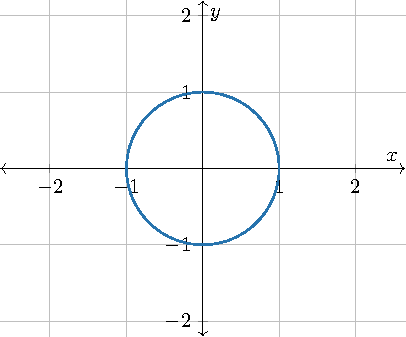
\includegraphics{chapters/2-RealAnalysis/figures/figures-parametriccircle.pdf}
    \end{center}

\end{example}


\begin{remark}
The two examples \hyperref[helix1]{$\bm{h}(t)$} and \hyperref[helix2]{$\bm{r}(s)$} show us that there are multiple possible parametrizations of the same curve.


\end{remark}

\begin{example}
The parametric curve of $\bm{h}(t) = \langle -\sin(t), \cos(t), t \rangle$ and $\bm{r}(s) = \langle -\sin(5s), \cos(5s), 5s \rangle$ is called a helix.


 \begin{center}        
        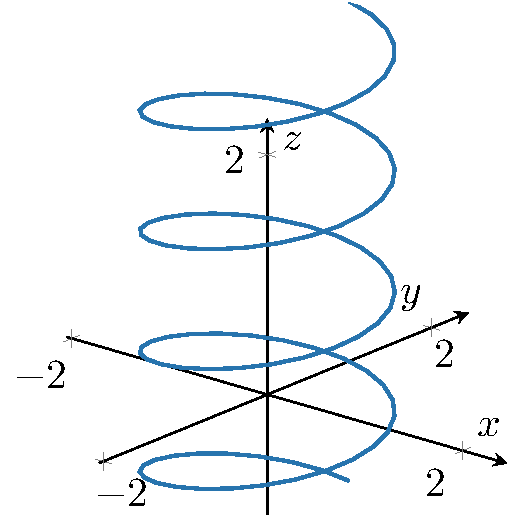
\includegraphics[scale=.75]{chapters/2-RealAnalysis/figures/figures-helixcurve.pdf}
    \end{center}

\end{example}


In other words, the parametrization describes how fast and in what direction you walk the path, whereas the parametric curve is the path itself.

\begin{motivating}
How can we sketch parametrizations and parametric curves?
\end{motivating}

Plotting points is something that a computer can do pretty easily\footnote{in fact, this is how all the graphics are plotted in these lecture notes!}; however, plotting points by hand is often a very inefficient way for humans to study parametric curves.  We will discuss two tools that can help us more easily sketch and understand vector-valued functions in $\R^3$.

\subsubsection{Projections}

Given a vector-valued function $\bm{r}(t) = \langle x(t), y(t), z(t) \rangle$, if we isolate and study the behavior of any two components, then we can gain information about the parametrization.

\begin{definition}
Given a vector-valued function $\bm{r}(t) = \langle x(t), y(t), z(t) \rangle$, we can study the following \textbf{projections}:

\begin{itemize}
    \item The projection onto the $xy$-plane, which corresponds to $\bm{r}(t) = \langle x(t), y(t), 0 \rangle$
    \item The projection onto the $xz$-plane, which corresponds to $\bm{r}(t) = \langle x(t), 0, z(t) \rangle$
     \item The projection onto the $yz$-plane, which corresponds to $\bm{r}(t) = \langle 0, y(t), z(t) \rangle$
\end{itemize}

\end{definition}

That is, we can think of these as shadows of the vector-valued function $\bm{r}(t)$.

\begin{example}
Consider the helix parametrization $\bm{h}(t) = \langle t, \cos(t), \sin(t) \rangle$ in $\R^3$.

\begin{itemize}
    \item The projection onto the $xy$-plane corresponds to $\bm{r}(t) = \langle t, \cos(t), 0 \rangle$.  This corresponds to a cosine curve in the $z=0$ plane, depicted on the bottom, in red.
    \item The projection onto the $xz$-plane corresponds to $\bm{r}(t) = \langle t, 0, \sin(t)\rangle$.  This corresponds to a sine curve in the $x=0$ plane, depicted on the right in orange.
    \item The projection onto the $yz$-plane corresponds to $\bm{r}(t) = \langle 0, \cos(t), \sin(t) \rangle$.  This describes counterclockwise motion around the unit circle centered at the origin, in the $yz$-plane, depicted on the left in green.  
\end{itemize}

\begin{center}
    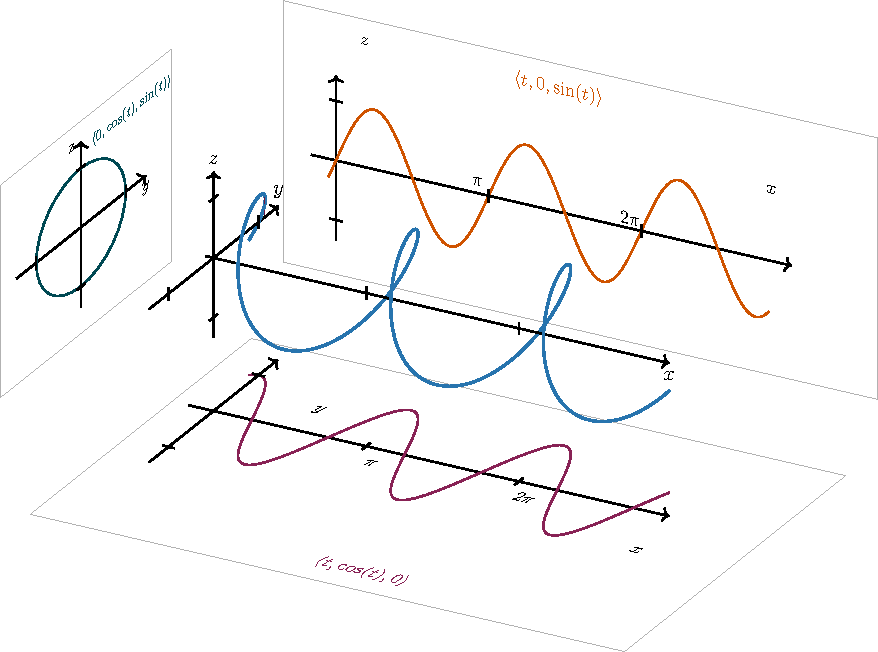
\includegraphics{chapters/2-RealAnalysis/figures/figures-projections.pdf}
\end{center}

\end{example}





\subsubsection{Quadric surfaces in $\R^3$}

Another tool we can use to graph and sketch vector-valued functions in $\R^3$ are called quadric surfaces:  These are certain well-studied surfaces in $\R^3$, that have been completely classified.


\begin{definition}
A \textbf{quadric surface}\define{quadric surface} in $\R^3$ is defined as the set of points $$\{ (x, y, z) \ | \ Ax^2 + By^2 + Cz^2 + Dxy + Exz + Fyz + ax + by + cz + d = 0\}$$
\end{definition}

\begin{example}
A plane of the form $ax + by + cz + d = 0$ is a quadric surface.
\end{example}

Thus, studying these quadric surfaces is a generalization of our discussion of planes.  We are now allowing for non-linear behavior!

\fixthis{say more}

Let us investigate a few non-linear examples:

\begin{example}
Let us consider the quadric surface $C$ given by  $$C := \{ (x, y, z) \ | \ x^2 + y^2 = 1\}$$

Observe that if we restrict our attention to the points that lie in both $C$ and in the plane $z = 0$, we see that these points can be described precisely as a unit circle centered at the origin, in the $z=0$ plane.

$$\{ (x, y, 0) \ | \ x^2 + y^2 = 1\}$$

Furthermore, this same picture holds if we instead consider any plane of the form $z=k$!  We again see a unit circle centered at the origin, but now in the $z=k$ plane.

$$\{ (x, y, k) \ | \ x^2 + y^2 = 1\}$$

Thus, the surface $C$ consists of a collection (one for each $k \in \R$) of unit circles centered at the origin, stacked on top of each other.  In other words, $C$ is an infinite cylinder of radius 1.
\end{example}

\fixthis{define cylinders}

We can use this technique in general to study the solutions to an arbitrary equation in $\R^3$ \fixthis{ref later}

\begin{definition}
    The \textbf{trace in the plane $P$}\define{trace} of a subset $S \subset \R^3$ is the intersection of $S$ with $P$.  That is, 
    $$S \cap P = \{\bm{x} \in \R^3 \ | \ \bm{x} \in S \ \textnormal{and} \ \bm{x} \in P\}$$
    
    We typically study $x$-traces, $y$-traces, and $z$-traces - that is, traces in the planes $x=k$, $y=k$, and $z=k$ respectively.
    
\end{definition}

We can think of traces as being slices of the graph. \fixthis{say more}


\begin{theorem}\label{quadraticcylinders}
Up to rotation and translation, there are 3 types of quadratic cylinders:

\begin{itemize}
    \item Parabolic cylinders, which have standard form $$y = \left(\frac{x}{a}\right)^2$$
    \item Elliptic cylinders, which have standard form $$\left(\frac{x}{a}\right)^2 + \left(\frac{y}{b}\right)^2 = 1$$
    \item Hyperbolic cylinders , which have standard form $$\left(\frac{x}{a}\right)^2 - \left(\frac{y}{b}\right)^2 = 1$$
\end{itemize}

\end{theorem}







\begin{theorem}
Up to rotation and translation, there are 8 types of quadric surfaces:

\begin{itemize}
    \item Planes, which have standard form $$ax + by + cz = d$$
    \item Quadratic cylinders (described in theorem \ref{quadraticcylinders}).
    \item Elliptic paraboloids, which have standard form $$z = \left(\frac{x}{a}\right)^2 + \left(\frac{y}{b}\right)^2$$
    \item Hyperbolic paraboloids, which have standard form $$z = \left(\frac{x}{a}\right)^2 - \left(\frac{y}{b}\right)^2$$
    \item Ellipsoids, which have standard form $$\left(\frac{x}{a}\right)^2 + \left(\frac{y}{b}\right)^2  + \left(\frac{z}{c}\right)^2 = 1$$
    \item Elliptic cones, which have standard form $$\left(\frac{z}{c}\right)^2  = \left(\frac{x}{a}\right)^2 + \left(\frac{y}{b}\right)^2$$
    \item Hyperboloids of one sheet, which have standard form $$\left(\frac{z}{c}\right)^2 +1 = \left(\frac{x}{a}\right)^2 + \left(\frac{y}{b}\right)^2  = \left(\frac{z}{c}\right)^2 + 1 $$
    \item Hyperboloids of two sheets, which have standard form $$\left(\frac{z}{c}\right)^2 - 1 = \left(\frac{x}{a}\right)^2 + \left(\frac{y}{b}\right)^2$$
\end{itemize}
\end{theorem}

That is, given any quadric surface, corresponding to a quadratic equation $Ax^2 + By^2 + Cz^2 + Dxy + Exz + Fyz + ax + by + cz + d = 0$, one can rotate it and translate it so that the quadratic equation can be written in the standard form above.

\begin{center}
    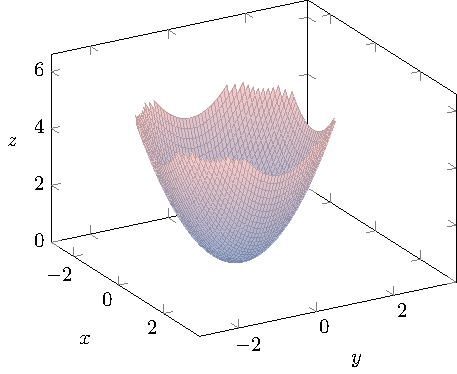
\includegraphics{chapters/2-RealAnalysis/figures/figures-ellipticparaboloid.pdf}
\end{center}

\begin{center}
    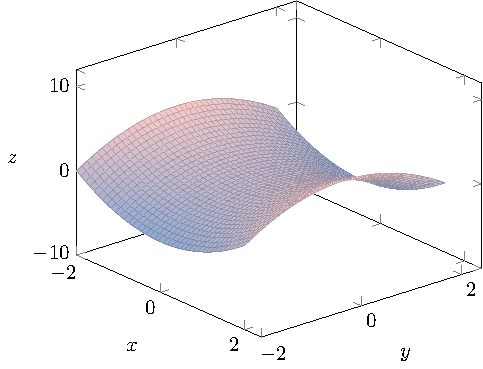
\includegraphics{chapters/2-RealAnalysis/figures/figures-hyperbolicparaboloid.pdf}
\end{center}

\begin{example}
The unit sphere of radius 1 in $\R^3$ can be described as the set of vectors $\{\bm{v} \in \R^3 \ | \ ||\bm{v}|| = 1\}$.  Equivalently, the unit sphere in $\R^3$ is the set of points $$\{ (x, y, z) \ | \ x^2 + y^2 + z^2 =1\}$$

Thus, the unit sphere of radius 1 is an example of an ellipsoid!
\end{example}

\begin{example}
Sketch and describe the surface $$x = \left(\frac{y-1}{4}\right)^2 + \left(\frac{z}{3}\right)^2 $$
\end{example}

\begin{example}
Describe and sketch the the quadric surface $S$ given by $$\frac{9(x-1)^2}{4}+4z^2 =9y^2 + 36$$
\end{example}


\begin{motivating}
How can we use this to sketch vector-valued functions?
\end{motivating}


Given a vector-valued function $\bm{r}(t) = \langle x(t), y(t), z(t) \rangle$, if we can find a relationship between the components of the coordinate vectors, then we know that $\bm{r}(t)$ must lie on the quadric surface.

\begin{example}
Consider the helix parametrization $\bm{h}(t) = \langle -\sin(t), \cos(t), t \rangle$ in $\R^3$.

Observe that the components of $\bm{h}(t)$ satisfy the equation $x(t)^2 + y(t)^2 = 1$.  This tells us indeed that the helix lies on the cylinder $x^2 + y^2 = 1$.

\fixthis{draw picture}
\end{example}



\subsection{Multivariable functions}\label{multivariablefunctions}

We now to turn to studying functions of the form $f : \R^n \to \R$:

\begin{definition}
A \textbf{multivariable function}\define{multivariable function} is a function $f : \R^n \to \R$.  We sometimes say that $f$ is a \textbf{function of $n$ variables}\define{function of $n$ variables}.
\end{definition}

\begin{example}
A scalar function $f : \R \to \R$ is a function of 1 variable.
\end{example}

\begin{example}
    The distance between the origin and a point $P = (x_1, \cdots, x_n)$  is a multivariable function $d : \R^n \to \R$ defined by 
    $$d(x_1, \cdots, x_n) = \sqrt{\sum_{i=1}^n x_i^2}$$
\end{example}

\begin{definition}
    Consider a subset $D \subset \R^n$.  The \textbf{indicator function} $1_D$ is the piecewise function defined by
    $$1_D(\bm{x}) := \left\{
		\begin{array}{ll}
			1 & \text{ if } \bm{x} \in D \\
			0 & \text{ if } \bm{x} \notin D
		\end{array}
		\right.$$
    
    \end{definition}



Just like with single-variable functions, we might be interested in functions that are defined only on a subset $D \subseteq \R^n$.  Nevertheless, the following construction shows us that it is sufficient to study the theory of multivariable functions $f : \R^n \to \R$.

\begin{example}
Let $D \subset \R^n$.  Then a function $f : D \to \R$ can be extended to a function of $n$ variables $\Tilde{f} : \R^n \to \R$ in the following way:
$$\Tilde{f}(\bm{x}) := \left\{
		\begin{array}{ll}
			f(\bm{x}) & \text{ if } \bm{x} \in D \\
			0 & \text{ if } \bm{x} \notin D
		\end{array}
		\right.$$

That is, to every point $\bm{x}=(x_1,\cdots,x_n)$ in the domain $D$, we assign the real number $f(\bm{x}) \in \R$.  To every other point $\bm{x} \notin D$, we assign the value $0$.  In other words,  $\Tilde{f}(\bm{x}) = f(\bm{x})1_D(\bm{x})$.  

\end{example}

\begin{motivating}
How should we geometrically interpret multivariable functions?
\end{motivating}

Recall that given a single variable function $f: \R \to \R$, we can draw its graph as the set of points $$\{(x, f(x)) \} \subseteq \R^2$$  We can generalize this to graph multivariable functions $f : \R^n \to \R$:

\begin{definition}\label{def:graph}
Given a function $f: \R^n \to \R$, its \textbf{graph}\define{graph of a multivariable function} is the following subset of $\R^{n+1}$:
$$\Gamma_f := \{(x_1,\cdots, x_n,f(x_1, \cdots, x_n)) \} \subset \R^{n+1}$$ 

In other words, the graph is given by the equation $$x_{n+1} = f(x_1, \cdots, x_n)$$ in $\R^{n+1}$.
\end{definition}

We can easily sketch and visualize graphs of functions with $2$ variables:

\begin{definition}
    The \textbf{graph} of a function of two variables $f(x,y)$ is the surface in $\R^3$ consisting of the set of points $(x,y,z)$ that are solutions to the equation
    $$z = f(x,y)$$
\end{definition}

\begin{motivating}
How can we sketch the graph of a function of two variables?
\end{motivating}

To sketch graphs in $\R^3$, we can again use traces!

\begin{definition}
    The \textbf{trace in the plane $P$}\define{trace} of a graph $\Gamma \subset \R^3$ is the intersection of $\Gamma$ with $P$.  That is, 
    $$\Gamma \cap P = \{\bm{x} \in \R^3 \ | \ \bm{x} \in \Gamma \ \textnormal{and} \ \bm{x} \in P\}$$
    
    We typically study $x$-traces, $y$-traces, and $z$-traces - that is, traces in the planes $x=k$, $y=k$, and $z=k$ respectively.
    
\end{definition}

We can think of traces as being slices of the graph. \fixthis{say more}

\begin{definition}
    The \textbf{level curves}\define{level curves} (isoclines, contour map) of a function of two variables $f(x,y)$ are the $z$-traces of the graph $z = f(x,y)$.
\end{definition}


\fixthis{picture}



\begin{example}
Sketch the graph of $f(x,y) = x^2 + y^2$.
\end{example}

\begin{example}
Sketch the graph of $f(x,y) = \sqrt{9-x^2 - y^2}$.
\end{example}



\subsubsection{Implicit functions}

From the previous section, we observed that some surfaces, such as the sphere in $\R^3$, are not graphs of multivariable functions.  That is, the sphere cannot be described as $z = f(x,y)$ for $f(x,y)$ a function of 2 variables. (As we will see later, they are graphs of multivariable functions \textbf{locally}).

Nevertheless, we can still describe them using multivariable functions implicitly!

\begin{definition}
Given a multivariable function $G(x_1, \cdots, x_n) : \R^n \to \R$, its \textbf{vanishing locus}\define{vanishing locus} is the set of points 
$$\{(x_1, \cdots, x_n) \ | \ G(x_1, \cdots, x_n) = 0\}$$
\end{definition}


\begin{example}
The unit sphere in $\R^3$ is the vanishing locus of the function $$G(x,y,z) = x^2 + y^2 +z^2-1$$
\end{example}

\begin{example}
All quadric surfaces are the vanishing loci of the general quadratic equation $$Q(x,y,z) = Ax^2 + By^2 + Cz^2 + Dxy + Exz + Fyz + ax + by + cz + d$$
\end{example}

We can also describe graphs of functions as vanishing loci!

\begin{example}
The graph of a multivariable function $x_{n+1}=f(x_1, \cdots, x_n)$ is the vanishing locus of the function $$G(x_1, \cdots, x_{n+1}) = f(x_1, \cdots, x_n) -x_{n+1}$$
\end{example}

Note that the vanishing locus of $G : \R^n \to \R$ is a subset of $\R^n$, whereas the graph of a function $f : \R^n \to \R$ is a subset of $\R^{n+1}$!  Again, this is analogous to the difference between the kernel of a linear map, versus the image of a linear map.






\subsection{General Multivariable functions}\label{generalmulti}

We now to turn to the general case:

\begin{definition}
A \textbf{general multivariable function}\define{general multivariable function} is a function $f : \R^n \to \R^m$, defined by 
$$f(x_1, \cdots, x_n) = \big\langle f_1(x_1, \cdots, x_n), f_2(x_1, \cdots, x_n), \cdots, f_m(x_1, \cdots, x_n) \big\rangle$$

\end{definition}

That is, a general multivariable function is a vector-valued function, whose components are multivariable functions!

\begin{example}
A vector-valued function is a general multivariable function $f : \R \to \R^m$.
\end{example}

\begin{example}
A multivariable function is a general multivariable function $f : \R^n \to \R$.
\end{example}


\subsection{Exercises}

\begin{problem}{Cycloid}

Consider the vector-valued function $\bm{r}(t) = \langle t-\sin(t), 1-\cos(t) \rangle$, which parametrizes a curve called a \textbf{cycloid}.  Sketch $\bm{r}(t)$ from $0$ to $2\pi$.

\end{problem}

\begin{problem}{swirly}
Sketch and describe the vector-valued function $\bm{r}(t) = \langle e^{-t}\sin(t), e^{-t}\cos(t), e^{-t} \rangle$.  

\begin{subproblems}
\item How many times does $\bm{r}(t)$ intersect a sphere of radius 1?
\end{subproblems}

\end{problem}

\begin{problem}{conicalhelix}
Sketch and describe the vector-valued function $\bm{r}(t) = \langle t\sin(t), t\cos(t), t \rangle$.  
\end{problem}

\begin{problem}{cylinderslice}
Find a parametrization of the intersection of the cylinder $x^2 + y^2 = 1$ and the plane $x + y + z = 1$.

Sketch and describe the parametric curve.
\end{problem}

\begin{problem}{cylinderparbola}
Find a parametrization of the intersection of the cylinder $x^2 + y^2 = 1$ and the parabolic cylinder $z = 4x^2$

Sketch and describe the parametric curve.
\end{problem}

\begin{problem}{Vistani1}
Vistani's curve is the intersection of the surfaces $x^2 + y^2 = z^2$ and $y=z^2$.  Find a parametrization of Vistani's curve.
\end{problem}

\begin{problem}{Vistani2}
Show that Vistani's curve lies on the unit sphere of radius 1, centered at $(0,1,0)$.
\end{problem}

\begin{problem}{inaplane}
    Show that the vector-valued function $\bm{r}(t) : \langle t^2-1, t-2t^2, 4-6t \rangle$ lies in a plane.  What is the equation of the plane?
\end{problem}

We say that two lines $\bm{r_1}(t)$ and $\bm{r_2}(s)$ \textbf{intersect} if there is a point $P$ lying on both curves.  We say that $\bm{r_1}(t)$ and $\bm{r_2}(s)$ \textbf{collide} if there exists some $t_0$ such that $\bm{r_1}(t_0) = \bm{r_2}(t_0)$.

\begin{problem}{colvsint}
What is the difference between a point of intersection and a point of collision?
\end{problem}

\begin{problem}{collision}
Consider the vector-valued functions $$\bm{r_1}(t) = \langle t^2 - 3, -1, t^2 \rangle \qquad \bm{r_2}(s) = \langle 2s, 2s+1, 2s+3 \rangle$$

\begin{subproblems}
\item Do $\bm{r_1}(t)$ and $\bm{r_2}(s)$ \textbf{collide}?  If so, find the point(s) of collision.
\item Find all values of $t$ and $s$ where the curves of $\bm{r_1}(t)$ and $\bm{r_2}(s)$ \textbf{intersect}.
\end{subproblems}

\end{problem}










\begin{problem}{traces1}
Sketch traces of the surface $x^2 + (\frac{y}{4})^2 + z^2 = 1$.
\end{problem}

\begin{problem}{quadricsurface1}
Classify and sketch the quadric surface $S$ given by $$\left(\frac{x}{2}\right)^2+\left(\frac{y}{5}\right)^2 =5z^2 - 1$$
\end{problem}

\begin{problem}{quadricsurface2}
Classify and sketch the quadric surface $S$ given by  $$9y^2+4\left(z-1\right)^2 =\frac{9x^2}{4} + 36$$
\end{problem}

\begin{problem}{traces2}
Sketch traces of the function $f(x,y) = \frac{y}{x^2}$.
\end{problem}

\begin{problem}{traces3}
Sketch traces of the function $f(x,y) = \frac{1}{x^2 + y^2 + 1}$.
\end{problem}

\begin{problem}{traces4}
Sketch traces of the function $f(x,y) = \cos(x-y)$.
\end{problem}

\begin{problem}{tracesinverse}
Consider the following equations:
    \begin{center}
    \def\arraystretch{1.5}
        \begin{tabular}{lc}
(i) & $\left(\frac{y}{2}\right)^2 =\left(\frac{x}{4}\right)^2 + \frac{8}{9}$                                         \\
(ii) & $\left(\frac{y}{2}\right)^2 =\left(\frac{x}{4}\right)^2 + 1$     \\
(iii) & $\left(\frac{y}{2}\right)^2+\left(\frac{z-1}{3}\right)^2 = 1$ 
\end{tabular}
    \end{center}
    
    \begin{subproblems}
    \item If a quadric surface $S$ has $(i)$ and $(ii)$ as traces, then can we determine $S$?
    \item If a quadric surface $S$ has $(i)$, $(ii)$, and $(iii)$ as traces, then can we determine $S$?
    \item If $(i)$ is a trace of a quadric surface $9y^2+4\left(z-1\right)^2 =\frac{9x^2}{4} + 36$, what plane could the trace be in?
    \item If $(iii)$ is a trace of a quadric surface $9y^2 + 4(z-1)^2 + 9(x-1)^2 = 36$, what plane could the trace be in?
    \end{subproblems}
    
\end{problem}


\begin{problem}{levelcurves1}
Sketch the level curves of the multivariable function $f(x,y) = |x| + |y|$
\end{problem}




\section{Limits of sequences}\label{sec:limits}

Now that we have a good understanding of multivariable functions, let us turn to rigorously studying limits and continuity in multivariable calculus.  We will first study limits of sequences (\hyperref[limseq]{of vectors}), and then turn to limits of functions (both \hyperref[limvectorval]{vector-valued} and \hyperref[limmulti]{multivariable} functions).

First, recall the notion of a limit of sequences of real numbers:

\begin{definition}
Let $\{a_k\}$ be a sequence of real numbers.  We say that the sequence \textbf{converges} if the following holds:

For all $\varepsilon>0$, there exists $M$ such that for all $m > M$, $$|a_m - L | < \varepsilon$$
    
We say $L$ is the \textbf{limit} of the sequence $\{a_k\}$.  If no such $L$ exists, we say $\{a_k\}$ \textbf{diverges}\define{sequence divergence}.
\end{definition}

In other words, the limit of a sequence $\{a_k\}$ is $L$ if for every small value $\varepsilon$, we can find an $M$ such that $a_m$ is $\varepsilon$-close to $L$ for $m > M$.



\begin{example}
Consider the sequence $\{\frac{1}{k^3 + 1}\}$.  Then $\lim_{k \to \infty} \frac{1}{k^3 + 1} = 0$.

\begin{proof}
Let $\varepsilon > 0$.  We wish to find $M$ such that for $m > M$, $|a_m - 0|  = a_m < \varepsilon$.

Let us choose $M > (\frac{1}{\varepsilon}-1)^{\frac{1}{3}}$.  Then if $m > M$, we have that $$m^3 > M^3 >  (\frac{1}{\varepsilon}-1)$$
Thus, $$m^3 +1  > \frac{1}{\varepsilon}$$
We can then deduce that for $m > M$,  $$\varepsilon > \frac{1}{m^3 +1} =a_m$$
That is, we have shown that $\lim_{k \to \infty} \frac{1}{k^3 + 1} = 0$.


\end{proof}

\end{example}





\begin{motivating}
Why do we need to use $\varepsilon$ when talking about limits?
\end{motivating}

Ideally, what we would like to say is that the sequence $\{a_k\}$ will eventually reach its limit, $L$.  However, if we consider the sequence $$\left\{\frac{1}{k^3 + 1}\right\}$$
We can observe that $\lim_{k\to \infty}\frac{1}{k^3 + 1} = 0$, but $\frac{1}{k^3 + 1} > 0$.

Thus, since the sequence $\{a_k\}$ might not ever attain its limit $L$, we need a different way to describe the limit:

\begin{proposition}\label{epsilonenough}
    Let $x \in \R_{\geq0}$.  Then the following are equivalent:
    
    \begin{enumerate}
        \item For all $\varepsilon >0$,  $x < \varepsilon$
        \item $x = 0$.
    \end{enumerate}
    \end{proposition}

As a consequence, to show that $a = b$, it is equivalent to show that there is no number between $a$ and $b$!


\begin{example}
Consider the sequence $\{\sum_{i=1}^k \frac{9}{10^i}\} = \{0.9, 0.99, 0.999, \cdots \}$.  Then $\lim_{k \to \infty} a_k = 1$.

In other words, the notion of limits explains why $0.\overline{999} = 1$.
\end{example}

Observe that in our definition, we use the term "\textbf{the} limit", which should imply that the limit of a sequence of real numbers is unique.  We verify that this is true:



\begin{proposition}[Limits are unique]\label{limsequnique1}
    Suppose $\{a_k\}$ is a sequence of real numbers that converges to both $a$ and $b$.  Then $a = b$.
    \end{proposition}

\begin{proof}
By proposition \ref{epsilonenough}, it is equivalent to show that for all $\varepsilon > 0$, $|a-b| < \varepsilon$.  Thus, let $\varepsilon > 0$.  

Since $\lim_{k \to \infty} a_k = a$, we know that there exists $M_a$ such that for all $m > M_a$, $|a_m -a| < \frac{\varepsilon}{2}$. Similarly, since $\lim_{k\to \infty} a_k = b$, we know that there exists $M_b$ such that for all $m > M_b$, $|a_m -b| < \frac{\varepsilon}{2}$.  Set $M = \textnormal{max}\{M_A, M_B\}$

Observe that $|a-b| = |a - a_m + a_m - b|$, and we can apply the triangle inequality to observe that for all $m > M$,
\begin{align*}
    |a-b| &= |a - a_m + a_m - b| \\
    & \leq |a-a_m| + |b-a_m| \\
    &< \frac{\varepsilon}{2} + \frac{\varepsilon}{2} = \varepsilon
\end{align*}

Thus, we have proven that for all $\varepsilon > 0$, $|a-b| < \varepsilon$.  Therefore, $a = b$, as desired.

\end{proof}


We can now rigorously prove the limit properties that we've seen in single variable calculus.


\begin{theorem}[Properties of Limits in $\R$]
    Let $\{a_k\}$ and $\{b_k\}$ be sequences in $\R$ that converge to $a$ and $b$, respectively. Then
    
    \begin{enumerate}
        \item $\lim_{k \to \infty}(a_k + b_k) = a + b$
        \item $\lim_{k \to \infty}\left(ca_k\right) = ca$ for all $c \in \R$.
        \item $\lim_{k \to \infty}\left(a_kb_k\right) = ab$.
        \item If $\{b_k\}, b \neq 0$, then $\lim_{k \to \infty}\frac{1}{b_k} = \frac{1}{b}$.
        \item If $\{b_k\}, b \neq 0$, then $\lim_{k \to \infty}\frac{a_k}{b_k} = \frac{a}{b}$.
    \end{enumerate}
    
    
    \end{theorem}
    
    
    
    
    
    

\begin{theorem}[Squeeze theorem for sequences]
    Let $\{a_k\}$, $\{b_k\}$, and $\{c_k\}$ be sequences in $\R$ such that there exists an $M$ such that $a_m \leq b_m \leq c_m$ for all $m > M$.  
    
    Then if $\lim_{k \to \infty}a_k = \lim_{k \to \infty}c_k = L$, then $\lim_{k \to \infty}b_k = L$.
    
\end{theorem}    
    
\begin{corollary}
    If $\lim_{k \to \infty} |a_k| = 0$, then $\lim_{k \to \infty}a_k = 0$.
\end{corollary}
    
    
    
    
    



\subsection{Limits of sequences of vectors}\label{limseq}

\begin{motivating}
How do we generalize the notion of sequences in $\R$ to sequences of vectors in $\R^k$?
\end{motivating}


Recall that the idea of a limit of a sequence of real numbers was the following:  $L$ is the limit of a sequence $\{a_n\}$ if for every small value $\varepsilon$, we can find an $N$ such that $a_n$ is $\varepsilon$-close to $L$ for $n > N$. 

The same idea should hold true for vectors in $\R^n$ - we We say that two points $\bm{P}, \bm{Q} \in \R^n$ are close to each other if the distance $||\bm{P-Q}||$ between them is small!


    \begin{definition}
    Let $\{\bm{a_n}\}$ be a sequence of vectors in $\R^k$.  We say that the sequence $\{\bm{a_n}\}$ \textbf{converges} to the vector $\bm{L} \in \R^k$ if:
    
    \vspace{1em}
    For all $\varepsilon>0$, there exists $M$ such that for all $m > M$, $$||\bm{a_m} - \bm{L} || < \varepsilon$$
    
    We say $\bm{L}$ is the limit of the sequence $\{\bm{a_n}\}$. If no such $\bm{L}$ exists, we say that $\{\bm{a_n}\}$ diverges.
\end{definition}

Another way to state the definition of limits is through topology:

\begin{definition}
    Let $\bm{P} \in \R^n$.  \textbf{The open ball of radius $\varepsilon$ around $\bm{P}$}\define{open ball}, denoted $B_{\varepsilon}(\bm{P})$, is the set of points 
    
    $$B_{\varepsilon}(\bm{P}) := \{ \bm{x} \in \R^n \ | \ ||\bm{x} - \bm{P} || < \varepsilon\}$$
    
    \end{definition}

    That is, $\lim_{n\to\infty} \bm{a_n} = \bm{L}$ if for every $\varepsilon > 0$, there is some $M$ such that $\bm{a_m} \in B_{\varepsilon}(\bm{L})$.

    \fixthis{picture}


Once again, we should confirm that the terminology "\textbf{the} limit" is correct.  The key idea of the proof is the same as in proposition \ref{limsequnique1}.

\begin{proposition}[Limits are unique]
    Suppose $\{\bm{a_n}\}$ converges to both $\bm{a}$ and $\bm{b}$ in $\R^n$.  Then $\bm{a} = \bm{b}$.
    \end{proposition}

\begin{proof}
By proposition \ref{epsilonenough}, it is equivalent to show that for all $\varepsilon > 0$, $||\bm{a}-\bm{b}|| < \varepsilon$.  Thus, let $\varepsilon > 0$.  

Since $\lim_{k \to \infty} \bm{a_k} = \bm{a}$, we know that there exists $M_a$ such that for all $m > M_a$, $||\bm{a_m} -\bm{a}|| < \frac{\varepsilon}{2}$. Similarly, since $\lim_{k\to \infty} \bm{a_k} = \bm{b}$, we know that there exists $M_b$ such that for all $m > M_b$, $||\bm{a_m} -\bm{b}|| < \frac{\varepsilon}{2}$.  Set $M = \textnormal{max}\{M_A, M_B\}$

Observe that $||\bm{a}-\bm{b}|| = ||\bm{a}-\bm{a_m}+\bm{a_m}-\bm{b}||$, and we can apply the triangle inequality to observe that for all $m > M$,
\begin{align*}
    ||\bm{a}-\bm{b}|| &= ||\bm{a}-\bm{a_m}+\bm{a_m}-\bm{b}|| \\
    & \leq ||\bm{a}-\bm{a_m}||+||\bm{a_m}-\bm{b}|| \\
    &< \frac{\varepsilon}{2} + \frac{\varepsilon}{2} = \varepsilon
\end{align*}

Thus, we have proven that for all $\varepsilon > 0$, $||\bm{a}-\bm{b}|| < \varepsilon$.  Therefore, $\bm{a} = \bm{b}$, as desired.

\end{proof}





\begin{theorem}[Limits in $\R^m$ are determined componentwise]\label{limseqcomponentwise}
    Let $\{\bm{a_n}\}$ be a sequence in $\R^m$, where $\bm{a_n} = \langle a_{n,1},\  a_{n,2},\  \cdots \ a_{n,m} \rangle$.
    
    \vspace{1em}
    
    Then $\{\bm{a_n}\}$ converges to $\bm{a} = \langle a_1, \cdots, a_m \rangle$ if and only if $\{a_{n,i}\}$ converges to $a_i$ for all $1 \leq i \leq m$.
    
    
    \end{theorem}

\begin{proof}
The key idea is the following inequalities $|a_{n,i} - a_i| \leq ||\bm{a_{n,i}} - \bm{a}|| \leq \sum_{i=1}^m |a_{n,i} - a_i|$.
\end{proof}



    \begin{corollary}
    Let $\{\bm{a_n}\}$ and $\{\bm{b_n}\}$ be sequences in $\R$ that converge to $\bm{a}$ and $\bm{b}$, respectively. Then
    
    \begin{enumerate}
        \item $\lim_{n \to \infty}(\bm{a_n} + \bm{b_n}) = \bm{a + b}$
        \item $\lim_{n \to \infty}\left(c\bm{a_n}\right) = c\bm{a}$ for all $c \in \R$.
    \end{enumerate}
    
    
    \end{corollary}







\subsection{Divergent sequences}




\begin{motivating}
Do limits of sequences always exist?
\end{motivating}

There are two main types of sequences that diverge:

    \begin{example}
    The sequence $\{(-1)^n\} = \{-1, 1, -1, 1 \cdots \}$ in $\R$ diverges.
    \end{example}
    
    \begin{example}
    The sequence $\{n\} = \{1, 2, 3, 4, \cdots\}$ in $\R$ diverges.
    \end{example}
    
    In this section, we will investigate the behavior of these sequences, and quantify why they don't converge.


\begin{definition}
    Let $\{\bm{a_n}\}$ be a sequence of vectors in $\R^k$.  A \textbf{subsequence} of $\{\bm{a_n}\}$ is a sequence $\{\bm{b_i}\}$, where $$\bm{b_i} = \bm{a_{n_i}}$$
    such that $n_1 < n_2 < \cdots < n_i < \cdots$.
    \end{definition}

    
    \begin{theorem}\label{subsequencediv}
    Let $\{\bm{a_n}\}$ be a sequence of vectors in $\R^k$ such that $\{\bm{a_n}\}$ has two different subsequences $\{\bm{a_{n_i}}\}$ and $\{\bm{a_{n_j}}\}$ that converge to two different limits.
    
    Then  $\{\bm{a_n}\}$ diverges.
    \end{theorem}
    
    
     \begin{example}
    The sequence $\{(-1)^n\}$ has the subsequences $$\{(-1)^{2n}\} = \{1, 1, 1, \cdots\}$$ and
    
    $$\{(-1)^{2n+1}\}= \{-1, -1, -1, \cdots\}$$ which converge to $1$ and $-1$, respectively.
    
    Hence $\{(-1)^n\}$ diverges by theorem $\ref{subsequencediv}$.
    \end{example}

    \fixthis{Can also prove it fails to follow definition}.

\begin{theorem}[Convergent sequences are bounded]

Let $\{\bm{a_n}\}$ be a sequence in $\R^k$ such that $\lim_{n \to \infty}\bm{a_n} = \bm{L}$.

\vspace{1em}

Then the sequence $\{\bm{a_n}\}$ is \textbf{bounded}.  That is, there exists a number $A \in \R$ such that $||\bm{a_n}|| \leq A$ for all $n$.
\end{theorem}
    
    \begin{proof}
    We would like to say that $A$ should be the largest value out of all the $||\bm{a_n}||$.  However, since the set $\{||\bm{a_n}||\}$ is an \textit{infinite} set, there does not necessarily exist a maximum.\footnote{The sequence $\{1-\frac{1}{n}\}$ has no maximal element, for example.  Nevertheless, it is still bounded!}

    However, we can take the maximum of a finite set!  Since $\lim_{n \to \infty}\bm{a_n} = \bm{L}$, if we choose $\varepsilon = 1$, then by definition, there exists $M$ such that for all $m > M$, $$||\bm{a_m} - \bm{L}|| < 1$$

    By the triangle inequality, this implies that $$||\bm{a_m}|| < ||\bm{L}|| + 1$$ for all $m > M$.

    Observe that the set $\{||\bm{a_1}||, \cdots, ||\bm{a_M}||, ||\bm{L}|| + 1 \}$ is finite, and we can then choose
    $$A = \textnormal{max}\{||\bm{a_1}||, \cdots, ||\bm{a_M}||, ||\bm{L}|| + 1 \}$$

    By construction, $||\bm{a_n}|| \leq A$ for all $n$, as desired.
    
    \end{proof}

    The essence of the proof can be summed up in the following picture:

    \begin{center}
        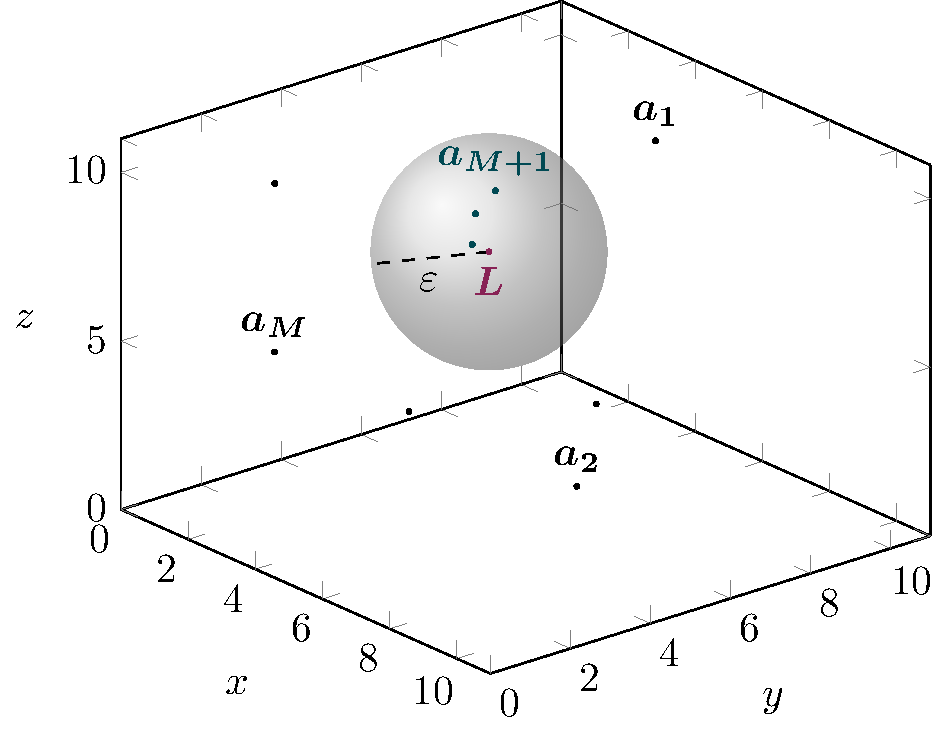
\includegraphics[scale=.5]{chapters/2-RealAnalysis/figures/figures-sequencebounded.pdf}
    \end{center}

    All vectors $\bm{a_m}$ for $m > M$ satisfy the property that $||\bm{a_m}|| \leq ||\bm{L}|| + \varepsilon$.  that is, those vectors are contained inside the small ball.  Outside of this ball, there are finitely many vectors.  Thus, if we take $A = \textnormal{max}\{||\bm{a_1}||, \cdots, ||\bm{a_M}||, ||\bm{L}|| + \varepsilon \}$, then we have bounded all the vectors in the sequence.
    
    
    \begin{corollary}
    If $\{\bm{a_n}\}$ be a sequence in $\R^k$ that is unbounded, then $\{\bm{a_n}\}$ diverges.
    \end{corollary}

\begin{example}
    The sequence $\{n\}$ in $\R$ is unbounded, hence it diverges.
    \end{example}



    It is not necessary that every term be unbounded - it's enough to find an unbounded subsequence!

\begin{theorem}\label{divergencecriteria}
Let $\{\bm{a_n}\}$ be a sequence of vectors in $\R^k$.  If $\{\bm{a_n}\}$ has a subsequence $\{\bm{a_{n_i}}\}$ that diverges, then $\{\bm{a_n}\}$ diverges.

\end{theorem}

\subsection{Exercises}
\begin{problem}{limitsdotprod}

Let $\{\bm{a_n}\}$ and $\{\bm{b_n}\}$ be sequences in $\R^n$ that converge to $\bm{a}$ and $\bm{b}$, respectively.  Show that
      \begin{enumerate}
          \item $\lim_{n \to \infty}( \bm{a_n} \cdot \bm{b_n} ) = \bm{a} \cdot \bm{b}$
          \item $\lim_{n \to \infty}(||\bm{a_n}||) = || \bm{a}||$
      \end{enumerate}
\end{problem}

\begin{problem}{limitsmagnitude}

Let $\{\bm{a_n}\}$ be a sequence in $\R^n$ that converges to $\bm{a}$.  Show that
      \begin{enumerate}
          \item $\lim_{n \to \infty}(||\bm{a_n}||) = || \bm{a}||$
      \end{enumerate}

\end{problem}

\begin{problem}{prodquotient}

Why don't we have product and quotient rules for limits of two sequences $\{\bm{a_n}\}$, $\{\bm{b_n}\}$ in $\R^n$?

\end{problem}

\begin{problem}{scalarprodquotient}
Conjecture and prove product and quotient rules for a sequence $\{\bm{a_n}\}$ in $\R^n$ and a sequence $\{b_n\}$ in $\R$.
\end{problem}

\begin{problem}{alternating}
Does the limit of the sequence $\{\frac{(-1)^n}{n}\}$ exist?  Prove your answer.
\end{problem}

\begin{problem}{limseqex1}
Does the limit of the sequence $\{\frac{n}{n+1}\}$ exist?  Prove your answer.
\end{problem}

% \begin{problem}
% Let $\{a_n\}$ and $\{b_n\}$ be sequences of real numbers.  
% Prove that if $\$

% there exists some $M$ such that  $a_m < b_m$ for all $m > M$
% \end{problem}

\begin{problem}{averages}

Let $\{\bm{a_n}\}$ be a sequence of real numbers.  The sequence of averages is the sequence $\{b_n\}$ defined by $$b_n = \frac{a_1 + \cdots + a_n}{n}$$

Prove that if $\lim_{n \to \infty} a_n = 0$, then the sequence of averages $\{b_n\}$ satisfies $\lim_{n \to \infty} b_n = 0$.

\end{problem}

\begin{definition}
Let $S$ be a non-empty subset of $\R$.  A real number $x$ is called an \textbf{upper bound}\SubIndex{upper bound} of $S$ if $x \geq s$ for all $s \in S$.
\end{definition}

\begin{definition}
Let $S$ be a non-empty subset of $\R$.  A real number $x$ is called the \textbf{least upper bound}\SubIndex{least upper bound} (alternatively, \textbf{supremum}\SubIndex{supremum}) of $S$ if
\begin{enumerate}
    \item $x$ is an upper bound for $S$
    \item If $y$ is an upper bound for $S$, then $x \leq y$
\end{enumerate}

We often write the least upper bound as $\textnormal{sup}(S)$
\end{definition}

It turns out that if $S$ is a non-empty subset of $\R$, then if $S$ has an upper bound, then S has a least upper bound. (see theorem \cref{thm:completness})

\begin{definition}
Let $S$ be a non-empty subset of $\R$.  A real number $x$ is called a \textbf{lower bound}\SubIndex{lower bound} of $S$ if $x \leq s$ for all $s \in S$.
\end{definition}

\begin{definition}
Let $S$ be a non-empty subset of $\R$.  A real number $x$ is called the \textbf{greatest lower bound}\SubIndex{greatest lower  bound} (alternatively, \textbf{infimum}\SubIndex{infimum}) of $S$ if
\begin{enumerate}
    \item $x$ is a lower bound for $S$
    \item If $y$ is a lower bound for $S$, then $x \geq y$
\end{enumerate}

We often write the greatest lower  bound as $\textnormal{inf}(S)$
\end{definition}

It turns out that if $S$ is a non-empty subset of $\R$, then if $S$ has a lower bound, then S has a greatest lower bound.


\begin{definition}
    A sequence of real numbers $\{a_n\}$ is said to be \textbf{increasing} (resp. \textbf{decreasing}) if $a_n \leq a_{n+1}$ (resp. $a_n \geq a_{n+1}$) for all $n$.
    \end{definition}
    
\begin{problem}{boundedincreasing}
Prove that if a sequence of real numbers $\{a_n\}$ is increasing and bounded above, then $\lim_{n \to \infty} a_n = \textnormal{sup}(\{a_n\})$
\end{problem}

\begin{problem}{boundeddecreasing}
Prove that if a sequence of real numbers $\{a_n\}$ is decreasing and bounded below, then $\lim_{n \to \infty} a_n = \textnormal{inf}(\{a_n\})$
\end{problem}


\begin{problem}{monotone}
Prove the following theorem:

Let $\{a_n\}$ be an increasing or a decreasing sequence.  Then $\{a_n\}$ converges if and only if $\{a_n\}$ is bounded.
\end{problem}

\section{Limits of functions}




Now let us turn to limits of functions!  Let us first recall the notion of limits of single-variable functions:


\begin{definition}
    A function $f :\R \to \R$ has the \textbf{limit} $b$ at $a$ if
    
    \vspace{1em}
    For all $\varepsilon>0$, there exists $\delta > 0$ such that for all $\bm{x} \in \R$, $$0 < |x-a| < \delta \qquad \textnormal{implies} \qquad |f(x) - b | < \varepsilon$$
    
    We write $\lim_{x \to a}f(x) = b$.
    
    \end{definition}


Since $\R$ is a well-ordered field (in other words, since ), we can turn this into a statement about left limits and right limits.

\fixthis{left and right picture}









\begin{definition}[Limit of a general multivariable function]
    A function $f : \R^n \to \R^m$ has the \textbf{limit} $\bm{b}$ at $\bm{a}$ if
    
    \vspace{1em}
    For all $\varepsilon>0$, there exists $\delta > 0$ such that for all $\bm{x} \in \R^n$, $$0 < ||\bm{x} - \bm{a} || < \delta \qquad \textnormal{implies} \qquad ||f(\bm{x}) - \bm{b} || < \varepsilon$$
    
    We write $\lim_{\bm{x} \to \bm{a}}f(\bm{x}) = \bm{b}$.
    
    \end{definition}


    \begin{proposition}[Limits of functions are unique]
    Let $f: \R^n \to \R^m$, and suppose $\lim_{\bm{x} \to \bm{a}}f(x) = \bm{b_1}$ and $\lim_{\bm{x} \to \bm{a}}f(x) = \bm{b_2}$.  Then $\bm{b_1} = \bm{b_2}$.
    \end{proposition}

We will study this for the two different classes of functions (\hyperref[limvectorval]{vector-valued functions} $\R \to \R^n$ and \hyperref[limmulti]{multivariable functions} $\R^n \to \R$)  we've seen.  This turns out to be enough, as we see in section \ref{limgenmulti}.














\subsection{Limits of vector valued functions}\label{limvectorval}

\begin{definition}[Limit of a vector-valued function]
    A function $f : \R \to \R^m$ has the \textbf{limit} $\bm{b}$ at $a$ if
    
    \vspace{1em}
    For all $\varepsilon>0$, there exists $\delta > 0$ such that for all $x \in \R$, $$0 < |x-a| < \delta \qquad \textnormal{implies} \qquad ||f(x) - \bm{b} || < \varepsilon$$
    
    \end{definition}


\begin{theorem}[Limits of vector-valued functions are determined componentwise]\label{vecvalcomponents}
    For any vector valued function $\bm{r}(t) = \langle x_1(t), \cdots, x_n(t) \rangle$, $$\lim_{t \to a} \bm{r}(t) = \langle x_1, \cdots, x_n \rangle$$ if and only if for all $1 \leq i \leq n$, $$\lim_{t \to a} x_i(t) = x_i$$
    
    
    \end{theorem}

    \begin{proof}
    The proof is essentially the same as the proof of theorem \ref{limseqcomponentwise}:
    
    The key idea is again the following inequalities $$|x_i(t) - x_i| \leq ||\bm{r}(t) - \langle x_1, \cdots, x_n \rangle|| \leq \sum_{i=1}^m |x_i(t) - x_i|$$
    
    
    
    \end{proof}

    
\fixthis{picture}


\begin{theorem}
    Let $\bm{r},\bm{s} : \R \to \R^m$ be vector-valued functions. Suppose that $\lim_{t \to a}\bm{r}(t)$ and $\lim_{t \to a}\bm{s}(t)$ exist. Then 
    
    \begin{enumerate}
        \item \textbf{Sum Law:} $$\lim_{t \to a} \left(\bm{r}(t) + \bm{s}(t))\right) = \lim_{t \to a} \bm{r}(t) + \lim_{t \to a} \bm{s}(t)$$
        \item \textbf{Scalar Multiple Law:} $$\lim_{t \to a} \lambda(\bm{r}(t)) = \lambda \left(\lim_{t \to a} \bm{r}(t) \right)$$
    \end{enumerate}
    
    
    \end{theorem}



\subsection{Limits of multivariable functions}\label{limmulti}

\begin{definition}[Limit of a multivariable function]
    A function $f : \R^n \to \R$ has the \textbf{limit} $b$ at $\bm{a}$ if
    
    \vspace{1em}
    For all $\varepsilon>0$, there exists $\delta > 0$ such that for all $\bm{x} \in \R^n$, $$0 < ||\bm{x} - \bm{a} || < \delta \qquad \textnormal{implies} \qquad |f(\bm{x}) - b | < \varepsilon$$
    \end{definition}

\begin{theorem}\label{limmultirules}
     Let $f,g : \R^n \to \R$ be functions of $n$ variables. Suppose that $\lim_{\bm{x} \to \bm{P}}f(\bm{x})$ and $\lim_{\bm{x} \to \bm{P}}g(\bm{x})$ exist. Then 
    
    \begin{enumerate}
        \item \textbf{Sum Law:} $$\lim_{\bm{x} \to \bm{P}} \left(f(\bm{x}) + g(\bm{x})\right) = \lim_{\bm{x} \to \bm{P}} f(\bm{x}) + \lim_{\bm{x} \to \bm{P}} g(\bm{x})$$
        \item \textbf{Scalar Multiple Law:} $$\lim_{\bm{x} \to \bm{P}} \lambda(f(\bm{x})) = \lambda \left(\lim_{\bm{x} \to \bm{P}} f(\bm{x}) \right)$$
        \item \textbf{Product Law:} $$\lim_{\bm{x} \to \bm{P}} \left(f(\bm{x})g(\bm{x})\right) = \left(\lim_{\bm{x} \to \bm{P}}f(\bm{x})\right)\left(\lim_{\bm{x} \to \bm{P}} g(\bm{x})\right)$$
        \item \textbf{Quotient Law:} If $\lim_{\bm{x} \to \bm{P}} g(\bm{x})\neq 0$, $$\lim_{\bm{x} \to \bm{P}} \frac{f(\bm{x})}{g(\bm{x})} = \frac{\lim_{\bm{x} \to \bm{P}}f(\bm{x})}{\lim_{\bm{x} \to \bm{P}} g(\bm{x})}$$
    \end{enumerate}
    
    
    \end{theorem}

This theorem allows us to reduce to studying limits of single-variable functions.
    
    \begin{example}
Let $f(x,y) = x$.  Then $$\lim_{(x,y) \to (a,b)}f(x,y) = a$$

\begin{proof}
Let $\varepsilon > 0$.  We wish to show that there exists $\delta > 0$ such that if $0 < ||(x,y) - (a,b) || < \delta$, then $|x-a| < \varepsilon$.

Observe that $$|x-a| = \sqrt{(x-a)^2} \leq \sqrt{(x-a)^2 +(y-b)^2} = ||(x,y) - (a,b) ||$$
Therefore, choosing $\delta = \varepsilon$, we see that if $||(x,y) - (a,b) || < \varepsilon$, then $|x-a| < \varepsilon$.

\end{proof}

\end{example}    


\begin{example}
Let $f(x,y) = \frac{x\sin(y)}{e^x+1}$.  Then $$\lim_{(x,y) \to (a,b)}f(x,y) = \frac{a\sin(b)}{e^a+1}$$
\end{example}  
    
    Observe that theorem \ref{limmultirules} allows us to evaluate the limits, except when we possibly divide by zero.
    
  \begin{motivating}
  When do limits of multivariable functions \textbf{not} exist?
  \end{motivating}  
    
    \begin{definition}
    Let $X \subset \R^n$.  We say that a point $\bm{p} \in \R^n$ is a \textbf{limit point of} $X$ if there is a sequence $\{\bm{a_n}\}$ contained inside $X$ such that $\{\bm{a_n}\}$ converges to $\bm{p}$.    
    \end{definition}
        
    
    \begin{theorem}
     Let $X \subset \R^n$, $f : X \to \R^m$ a function, and $\bm{a}$ a limit point of $X$.  Then the following statements are equivalent:
     
     \begin{enumerate}
         \item $\lim_{\bm{x} \to \bm{a}}f(x) = \bm{b}$
         \item For every sequence $\{\bm{a_n}\}$ converging to $\bm{a}$ (with $\bm{a_n} \neq \bm{a}$), the sequence $\{f(\bm{a_n})\}$ converges to $\bm{b}$.
     \end{enumerate}
     
    \end{theorem}
    
    In other words, in order for a limit of a multivariable function to exist, it must yield the same value \textbf{along all possible approaches}.
    
    \begin{example}
    Show that $\lim_{(x,y) \to (0,0)} \frac{x^2}{x^2 + y^2}$ does not exist.
    
    Consider the paths $\bm{r_1}(t) = \langle 0, t \rangle$, and $\bm{r_2}(t) = \langle t, t \rangle$.
    \end{example}
    
    
    \begin{motivating}
        What other tools can we use to prove limits exist?
    \end{motivating}
    
    It's often difficult to use epsilon-delta arguments to prove that limits exist (especially limits involving non-polynomial functions like $\sin(x), \cos(x)$, $e^x$, etc.).  Thus, we would like other ways to prove that limits exist.

    In these notes, we will discuss two tools that one can use:

       
    \begin{theorem}[Squeeze Theorem]
    Let $f(\bm{x})$, $g(\bm{x})$, and $h(\bm{x})$ be functions of $n$ variables such that $$\lim_{\bm{x} \to \bm{P}}f(\bm{x}) = L = \lim_{\bm{x} \to \bm{P}}h(\bm{x})$$
    
    If there exists $\delta > 0$ such that for all $\bm{x} \in B_\delta(\bm{P}) - \{\bm{P}\}$, we have that $$f(\bm{x}) \leq g(\bm{x}) \leq h(\bm{x})$$ 
    Then $\lim_{\bm{x} \to \bm{P}}g(\bm{x}) = L$.
    \end{theorem}

    

    
    \begin{example}
    Consider the limit $$\lim_{(x,y) \to (0,0)} x\sin(\frac{1}{x^2 + y^2})$$ 

    Observe that for all $\theta$,  $|\sin(\theta)| \leq 1$.  Therefore, it follows that $|x\sin(\frac{1}{x^2 + y^2})| \leq |x|$.  Thus, 
    $$-|x| \leq x\sin(\frac{1}{x^2 + y^2}) \leq |x|$$
    Since we know that $\lim_{(x,y) \to (0,0)} -|x| = \lim_{(x,y) \to (0,0)} |x| = 0$, by the squeeze theorem it follows that $$\lim_{(x,y) \to (0,0)} x\sin(\frac{1}{x^2 + y^2}) = 0$$ 
    \end{example}
    

    We can also use polar coordinates to compute limits of functions in two variables.  The key idea is the following proposition:

\begin{proposition}

If we set $x = r\cos(\theta)$, $y  = r\sin(\theta)$, then $(x,y)$ approaches $(0,0)$ if and only if $r$ approaches $0$.

\end{proposition}

So if we have a a limit of a function of two-variables $\lim_{(x,y) \to (0,0)} f(x,y)$, we can often use polar coordinates to \textbf{try} to reduce our limit to a single-variable limit, by considering the function $$g(r,\theta) = f(r\cos(\theta), r\sin(\theta))$$ and studying the limit 
$$\lim_{r \to 0} g(r,\theta)$$

\begin{example}
    Consider the limit $$\lim_{(x,y) \to (0,0)} \frac{x^2y}{x^2+y^2}$$  
    
    Upon converting to polar coordinates, we obtain 
    \begin{align*}
        \lim_{(x,y) \to (0,0)} \frac{x^2y}{x^2+y^2} &= \lim_{r \to 0} \frac{(r\cos(\theta))^2r\sin(\theta)}{(r\cos(\theta))^2 + (r\sin(\theta))^2} \\
        &= \lim_{r \to 0} \frac{r^3\cos^2(\theta)\sin(\theta)}{r^2} \\
        &= \lim_{r \to 0}r\cos^2(\theta)\sin(\theta) 
    \end{align*}

    Observe that since both $|\cos(\theta)| \leq 1$ and $|\sin(\theta)| \leq 1$, we can conclude that $|r\cos^2(\theta)\sin(\theta)| \leq |r|$.  Thus,
    
    $$\lim_{(x,y) \to (0,0)} \left|\frac{x^2y}{x^2+y^2}\right| \leq \lim_{r \to 0} |r| = 0$$
    
    So by the squeeze theorem, we can conclude that $$\lim_{(x,y) \to (0,0)} \frac{x^2y}{x^2+y^2} = 0$$  
\end{example}

However, converting to polar coordinates will not always be successful, as you will see in the exercises below \fixthis{REFERENCE}.  A precise statement about limits in polar coordinates is as follows:

    
    \begin{theorem}[Limits using polar coordinates]\label{thm:polarlim}
    Let $f(x,y) : \R^2 \to \R$ be a function of two variables, which we can express in polar coordinates as $g(r,\theta) := f(r\cos(\theta), r\sin(\theta))$.  Then $$\lim_{(x,y) \to (0,0)} f(x,y) = L$$ if and only if there exists $\delta > 0$ and a function $h : \R \to \R$ such that 
    
    \begin{itemize}
        \item If $0 < r < \delta$, then $|g(r,\theta) - L| \leq h(r)$ for all $\theta$, AND
        \item $\lim_{r\to0} h(r) = 0$
    \end{itemize}

    \end{theorem}

\begin{corollary}
    If $\lim_{r \to 0} g(r,\theta)$ depends on $\theta$, then the value of the limit will differ for different straight line paths.  Thus, $\lim_{(x,y) \to (0,0)} f(x,y)$ does not exist.
\end{corollary}
    
    
    
    
    

\subsection{Limits of general multivariable functions}\label{limgenmulti}
    
    Now that we have studied limits of both \hyperref[limvectorval]{vector-valued functions} $\R \to \R^n$ and \hyperref[limmulti]{multivariable functions} $\R^n \to \R$, this turns out to capture the behavior of limits of general multivariable functions $\R^n \to \R^m$!
    
    The key idea is the following theorem:
    
    \begin{theorem}[Limits of general multivariable functions are determined componentwise]\label{thm:genmultilimit}
    For any general multivariable function $f : \R^n \to \R^m$, defined by 
$$f(x_1, \cdots, x_n) = \big\langle f_1(x_1, \cdots, x_n), f_2(x_1, \cdots, x_n), \cdots, f_m(x_1, \cdots, x_n) \big\rangle$$
Then 
$$\lim_{\bm{x} \to \bm{P}} f(\bm{x}) = \langle b_1, \cdots, b_n \rangle$$ if and only if for all $1 \leq i \leq m$, $$ \lim_{\bm{x} \to \bm{P}} f_i(\bm{x}) = b_i$$

    \end{theorem}
    
    \begin{proof}
    The proof idea is exactly the same as theorem \ref{vecvalcomponents}.
    \end{proof}
    
    Thus, it is indeed enough to study limits of multivariable functions $\R^n \to \R$.
    
    
    
    
    

\subsection{Exercises}



\begin{problem}{lim0}
Show that $\lim_{(x,y) \to (0,0)} x\sin(\frac{1}{x^2 + y^2}) =0$.
\end{problem}

\begin{problem}{lim15}
Show that $\lim_{(x,y) \to (0,0)} \frac{y^2}{x^2 + y^2}$ does not exist.
\end{problem}

\begin{problem}{limsqueeze}
Use the squeeze theorem to compute $\lim_{(x,y) \to (0,0)} \frac{5xy^2}{x^2+y^2}$
\end{problem}

\begin{problem}{lim5}
Show that the following limit does not exist.
     $$\lim_{(x,y) \to (0,0)} \frac{xy^2}{x^2 + 3y^4}$$
\end{problem}

\begin{problem}{lim1}
$\lim_{(x,y) \to (1,2)} x^2+y$ exist? Prove or disprove your claim.
\end{problem}

\begin{problem}{lim2}
Does $\lim_{(x,y) \to (0,0)} \frac{xy}{x^2 + y^2}$ exist? Prove or disprove your claim.
\end{problem}

\begin{problem}{lim3}
Does $\lim_{(x,y,z) \to (0,0,0)} \frac{x + y+ z}{x^2 + y^2 +z^2}$ exist? Prove or disprove your claim.
\end{problem}

\begin{problem}{lim4}
Does $\lim_{(x,y,z) \to (0,0,0)} \frac{xyz}{x^3 + y^3 +z^3}$ exist? Prove or disprove your claim.
\end{problem}

\begin{problem}{sequenceofpoints}
Consider the function $f(x,y) = \left\{
		\begin{array}{ll}
			\cos(x) & \text{ if } x^2 + y^2 = \frac{1}{n} \text{ for some } n = 1, 2, 3, \dots \\
			0 & \text{ otherwise } 
		\end{array}
		\right.$
		
		Compute $\lim_{(x,y) \to (0,0)} f(x,y)$ or show that it does not exist.	
\end{problem}

\begin{problem}{sequenceofpoints2}
    Consider the function $$f(x,y) = \left\{
		\begin{array}{ll}
			1 & \text{ if } (x,y) \neq (0,0) \textnormal{ with } x+y \textnormal{ rational} \\
			0 & \text{ if } (x,y) \neq (0,0) \textnormal{ with } x+y \textnormal{ irrational} \\
			1 & \text{ if } (x,y) = (0,0)
		\end{array}
		\right.$$
		
		Compute $\lim_{(x,y) \to (0,0)} f(x,y)$ or show that it doesn't exist.
\end{problem}

\begin{problem}{polarpoint}
    We can use polar coordinates to compute limits of functions in two variables approaching the point $(0,0)$.  How can we modify the polar coordinate method to compute limits of functions in two variables approaching the point $(a,b)$?
\end{problem}

\begin{problem}{polar1}
    Use polar coordinates to show that the limit $\lim_{(x,y) \to (0,0)} \frac{x^2}{x^2+y^2}$ does not exist.
\end{problem}

\begin{problem}{polarvsreg1}
    Convert the limit $\lim_{(x,y) \to (0,0)} \frac{x^2y}{x^4+y^2}$ to polar coordinates, and show that for all $\theta$, $\lim_{r\to0} g(r, \theta) = 0$.
\end{problem}

\begin{problem}{polarvsreg2}
    Show that $\lim_{(x,y) \to (0,0)} \frac{x^2y}{x^4+y^2}$ doesn't exist by finding two paths $\bm{r_1}(t)$ and $\bm{r_2}(t)$, passing through the origin, such that the limit of $f(x,y)$ along these two paths have different values.  
\end{problem}

\begin{problem}{polarvsreg3}
    Why do your answers in exercises \ref{problem:polarvsreg1} and \ref{problem:polarvsreg2} not contradict each other?  How do they relate to theorem \ref{thm:polarlim}?

\end{problem}


\section{Continuity}\label{sec:continuity}

Let us now turn to continuity.  Let us first recall the notion of continuity for a single-variable function:


\begin{definition}
    A function $f :\R \to \R$ is continuous at $a \in \R$ if $\lim_{x \to a}f(x) = f(a)$.
    
    \end{definition}

That is, the limit of the function at $a$ is precisely the value of the function at $a$.

\fixthis{picture}


The idea for general multivariable functions is identical:

\begin{definition}
    A general multivariable function $f: \R^m \to \R^n$ is \textbf{continuous} at a point $\bm{P} \in \R^m$ if 
    $$\lim_{\bm{x} \to \bm{P}} f(\bm{x}) = f(\bm{P})$$
    
    $f$ is said to be continuous on a subset $X \subset \R^m$ if it is continuous for every $\bm{P} \in X$.
    
    \end{definition}

That is, the limit of the function at $\bm{P}$ is precisely the value of the function at $\bm{P}$.

Thus, questions about continuity are really questions about limits:  To show that a function is continuous, you need to show that the limit exists, and then check that the limit matches the value of the function.

Thus, all of our theorems about limits immediately yield theorems about continuity.

\begin{theorem}
    Suppose $f: \R^m \to \R^n$ and $g: \R^m \to \R^n$ are general multivariable functions that are \textbf{continuous} at a point $\bm{P}$. Then
    
    \begin{enumerate}
        \item \textbf{Sum Law:} $f+g$ is continuous at $\bm{P}$.
        \item \textbf{Scalar Multiple Law:} $\lambda f$ is continuous at $\bm{P}$.

    \end{enumerate}
    
    
    \end{theorem}

\subsection{Vector-valued functions}

\begin{proposition}
   For any vector valued function $$\bm{r}(t) = \langle x_1(t), \cdots, x_n(t) \rangle$$ 
   $\bm{r}(t)$ is continuous at $P$ if and only if for all $1 \leq i \leq n$, $x_i(t)$ is continuous at $P$.
    \end{proposition}


    \subsection{Multivariable functions}

\begin{theorem}[Properties of continuity of multivariable functions]\label{sumscalarmultcont}
     Let $f,g : \R^n \to \R$ be functions of $n$ variables. Suppose that $f(\bm{x})$ and $g(\bm{x})$ are continuous at $\bm{P}$.
    
    \begin{enumerate}
        \item \textbf{Product Law:} $f(\bm{x})g(\bm{x})$ is continuous at $\bm{P}$.
        \item \textbf{Quotient Law:} If $g(\bm{P})\neq 0$, $\frac{f(\bm{x})}{g(\bm{x})}$  is continuous at $\bm{P}$.
    \end{enumerate}
    
    
    \end{theorem}

    \begin{example}
    The function $f: \R^2 \to \R$ given below is continuous for all $(x,y) \in \R^2$. $$f(x,y) = \left\{
		\begin{array}{ll}
			\frac{xy^2}{x^2 + y^2} & \text{ if } (x,y) \neq \bm{0} \\
			0 & \text{ if } (x,y) = \bm{0}
		\end{array}
		\right.$$
		
	\begin{proof}
	By the quotient law, $f$ is continuous for all $(x,y) \neq 0$.  We thus only need to show that $\lim_{(x,y) \to (0,0)} \frac{xy^2}{x^2 + y^2} = 0$
	
	We will show this directly, but we could have also used the squeeze theorem, or the polar coordinates method.
	
	Let $\varepsilon > 0$.  We need to find $\delta > 0$ such that if $0 < ||\langle x, y \rangle|| < \delta$, then $$|\frac{xy^2}{x^2 + y^2} - 0| < \varepsilon$$
	
	Observe that since $x^2 > 0$, then $$|\frac{xy^2}{x^2 + y^2}| \leq |\frac{xy^2}{y^2}| = |x|$$
	
	Thus, if we choose $\delta = \varepsilon$, then we know that $|x| \leq ||\langle x, y \rangle|| < \varepsilon$.  Hence $|\frac{xy^2}{x^2 + y^2}| \leq |\frac{xy^2}{y^2}| = |x| < \varepsilon$, as desired.
	
	\end{proof}
		
    \end{example}

    \begin{theorem}[The composition of continuous functions is continuous.]
    Let $f : \R^n \to \R^m$, and let $g: \R^m \to \R^k$ be multivariable functions such that $f$ is continuous at $\bm{P} \in \R^n$, and $g$ is continuous at $f(\bm{P}) \in \R^m$.
    
    \vspace{1em}
    Then $g \circ f : \R^n \to \R^k$ is continuous at at $\bm{P} \in \R^n$.
    \end{theorem}
    
    \begin{proof}
    \fixthis{do proof}
    \end{proof}
    
    \begin{theorem}
    $\det : M_{n \times n}(\R) \cong \R^{n^2} \to \R$ is continuous.
    \end{theorem}
    
    \begin{corollary}
    The cross product $\times : \R^3 \to \R^3 \to \R^3$ is continuous.
    \end{corollary}
    
    
    
    \begin{theorem}
    Let $T: \R^n \to \R^m$ be a linear map.  Then $T$ is continuous (in fact, $T$ is uniformly continuous).
    \end{theorem}
    
    \begin{definition}
    A multivariable function $f : \R^n \to \R^m$ is \textbf{uniformly continuous}\define{uniformly continuous} if 
    
    \vspace{1em}
    For all $\varepsilon>0$, there exists $\delta > 0$ such that for all $\bm{a}, \bm{b} \in X$, $$0 < ||\bm{a} - \bm{b} || < \delta \qquad \textnormal{implies} \qquad ||f(\bm{a}) - f(\bm{b}) || < \varepsilon$$
    
    \end{definition}
    
    
    
\subsection{Exercises}

\begin{problem}{cont0}
Consider the function  $f(x,y) = \left\{
		\begin{array}{ll}
			y^2\sin(\frac{1}{(x-4)^2 + y^2}) & \text{ if } (x,y) \neq (4,0) \\
			c & \text{ otherwise } 
		\end{array}
		\right.$
		
		Either show that there is a $c$ that will make $f$ continuous at $(4,0)$, or show that $f$ will not be continuous for any choice of $c$.
\end{problem}

\begin{problem}{cont1}
Consider the function $f(x,y) = \left\{
		\begin{array}{ll}
			\frac{x^2 + \sin(y)}{2x^2 + y +e^{xy}-1} & \text{ if } (x,y) \neq (0,0) \\
			1 & \text{ otherwise } 
		\end{array}
		\right.$
		
		Is $f$ continuous at $(0,0)$?
\end{problem}



\begin{problem}{cont2}
Consider the function  $f(x,y) = \left\{
		\begin{array}{ll}
			\frac{x^2  +\sin(xy)+y^2}{2x^2 + y^2} & \text{ if } (x,y) \neq (0,0) \\
			c & \text{ otherwise } 
		\end{array}
		\right.$
		
		Either show that there is a $c$ that will make $f$ continuous, or show that $f$ will not be continuous for any choice of $c$.
\end{problem}

\begin{problem}{cont3}
Consider the function $f(x,y) = \left\{
		\begin{array}{ll}
			\frac{y^5}{x^4 + y^4} & \text{ if } (x,y) \neq (0,0) \\
			1 & \text{ otherwise } 
		\end{array}
		\right.$
		
		Is $f$ continuous at $(0,0)$?
\end{problem}

\begin{problem}{cont4}
Consider the function  $g(x,y) = \left\{
		\begin{array}{ll}
			x^2\cos(\frac{1}{x^2 + y^2}) & \text{ if } (x,y) \neq (0,0) \\
			c & \text{ otherwise } 
		\end{array}
		\right.$
		
		Either show that there is a $c$ that will make $g$ continuous, or show that $g$ will not be continuous for any choice of $c$.
\end{problem}

\begin{problem}{cont5}
Consider the function  $f(x,y) = \left\{
		\begin{array}{ll}
			\frac{x^2}{x^2 + |y|^3} & \text{ if } (x,y) \neq (0,0) \\
			c & \text{ otherwise } 
		\end{array}
		\right.$
		
		Either show that there is a $c$ that will make $f$ continuous at $(0,0)$, or show that $f$ will not be continuous for any choice of $c$.
\end{problem}

\begin{problem}{cont6}

Consider the function  $f(x,y) = \left\{
		\begin{array}{ll}
			x\sin(\frac{1}{x^2 + y^2}) & \text{ if } (x,y) \neq (0,0) \\
			c & \text{ otherwise } 
		\end{array}
		\right.$
		
		Either show that there is a $c$ that will make $f$ continuous at $(0,0)$, or show that $f$ will not be continuous for any choice of $c$.

\end{problem}

\begin{problem}{cont7}
Consider the function  $g(x,y) = \left\{
		\begin{array}{ll}
			\frac{x^4  +2x^2y^2 +y^4}{x^2 + y^2} & \text{ if } (x,y) \neq (0,0) \\
			c & \text{ otherwise } 
		\end{array}
		\right.$
		
		Either show that there is a $c$ that will make $g$ continuous at $(0,0)$, or show that $g$ will not be continuous for any choice of $c$.
\end{problem}

\begin{definition}
A function $f : \R^n \to \R^m$ is said to be \textbf{Lipschitz} it there exists a constant $K \geq 0$ such that for all $\bm{x_1},\bm{x_2} \in \R^n$,  $$||f(\bm{x_1}) - f(\bm{x_2})|| \leq K ||\bm{x_1} - \bm{x_2}|| $$
\end{definition}

\begin{problem}{Lipschitz}

    Prove that if a function $f : \R^m \to \R^n$ is Lipschitz, then $f$ is continuous.

\end{problem}
    